\subsection{Web application}
	La componente \textit{web app} ha il compito di interfacciare gli utenti con i dispositivi censiti dal sistema e visibili al loro ente di appartenenza.
	\newline
	Le principali funzionalità messe a disposizione riguardano la visualizzazione di grafici contenenti i dati di determinati sensori, la modifica delle configurazioni dei gateway e l'aggiunta o la rimozione di dispositivi e/o sensori.
	\newline 
	La componente è stata sviluppata utilizzando i framework Laravel e Vue.js.
	
	\subsubsection{Diagramma dei package}%%%%%%%%%OK
		\begin{figure}[H]
			\centering
			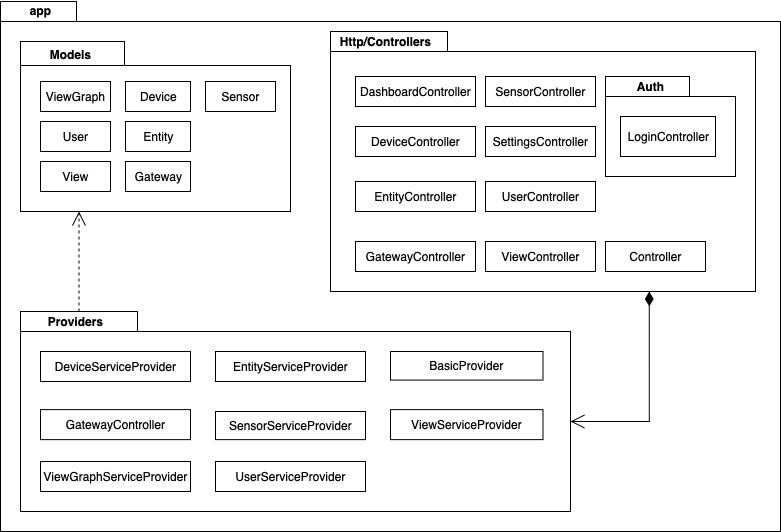
\includegraphics[scale=0.600]{res/images/WEBAPP/WebAppPackage.png}
			\caption{Diagramma dei package della componente web app}
			\label{Diagramma 21}
		\end{figure}

	\begin{landscape}
	\subsubsection{Diagrammi delle classi}%%%%%%%%%%OK
		\begin{figure}[H]
			\centering
			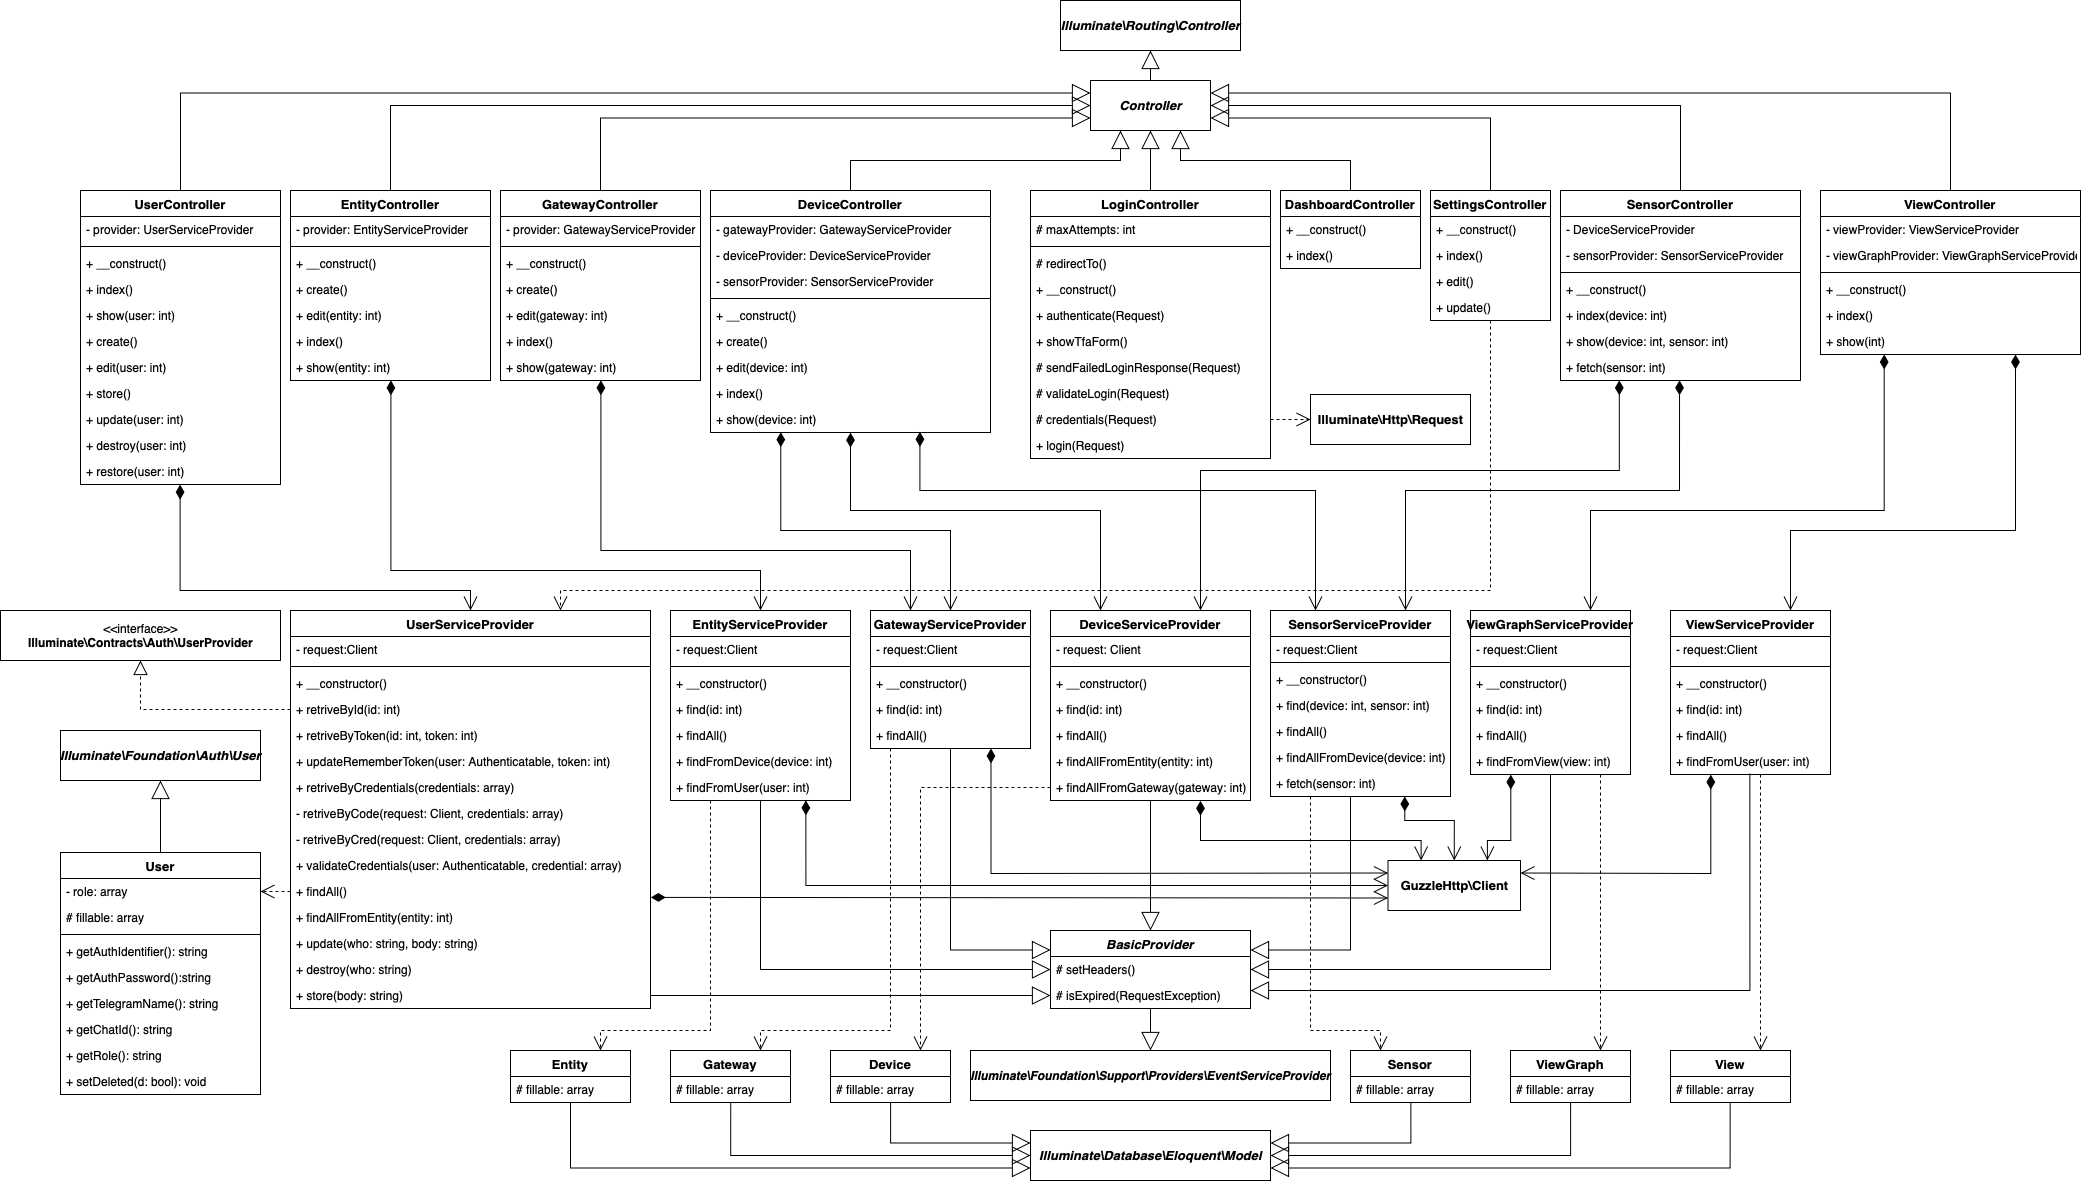
\includegraphics[scale=0.350]{res/images/WEBAPP/ClassiWebApp.png}
			\caption{Diagramma delle classi della componente web app}
			\label{Diagramma 22}
		\end{figure}
	\subsubsection{Diagrammi di sequenza}%%%%%%%%%%OK
		\begin{figure}[H]
			\centering
			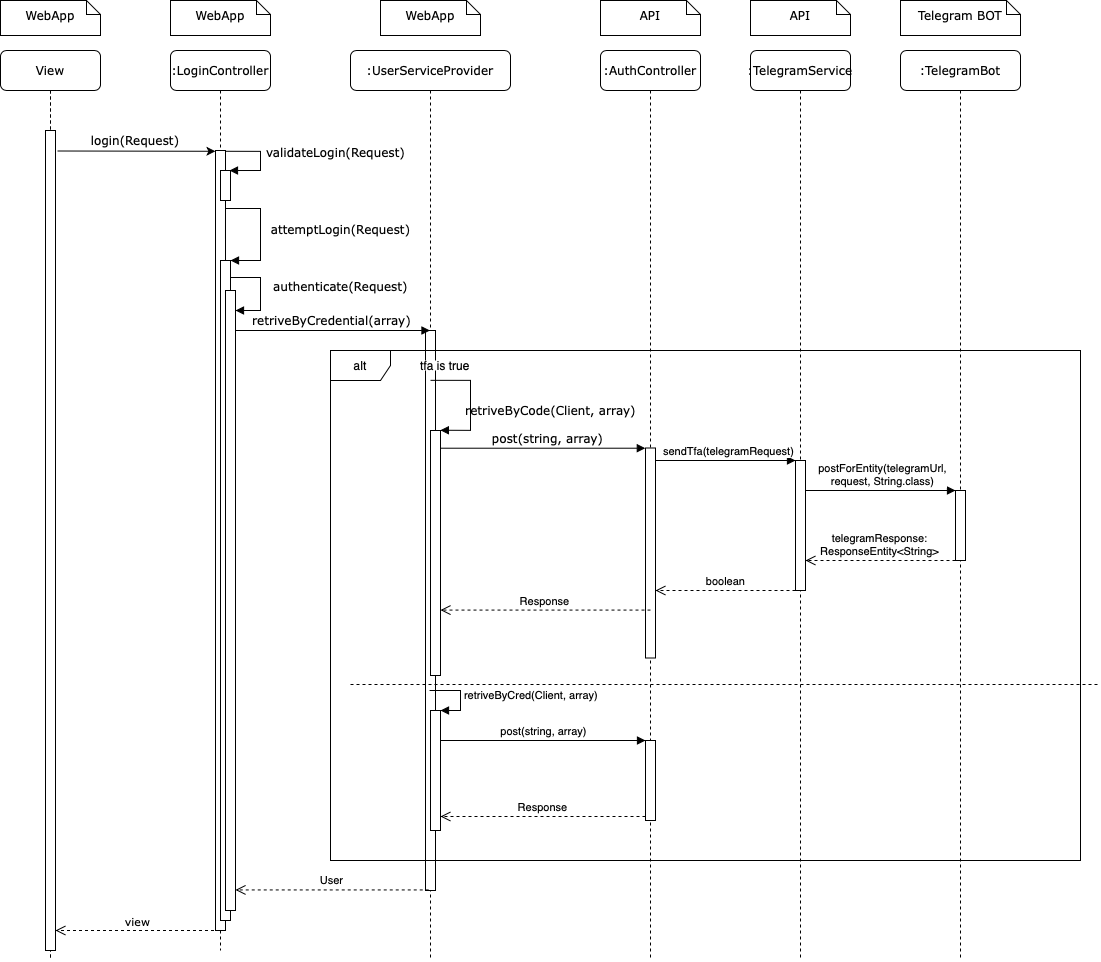
\includegraphics[scale=0.425]{res/images/WEBAPP/AutenticazioneTfa.png}
			\caption{Diagramma di sequenza che illustra l'autenticazione a due fattori all'interno della componente web app}
			\label{Diagramma 23}
		\end{figure}
		\begin{figure}[H]
			\centering
			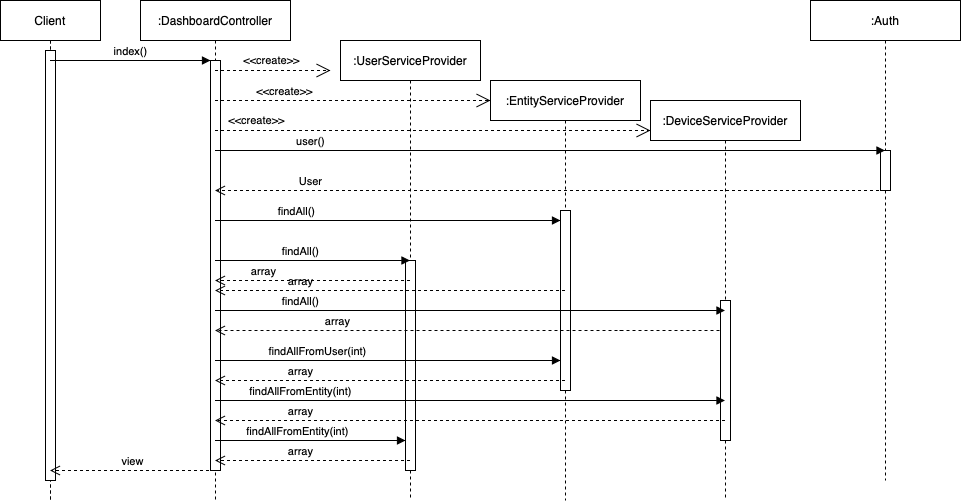
\includegraphics[scale=0.600]{res/images/WEBAPP/Dashboard.index.png}
			\caption{Diagramma di sequenza che illustra la visualizzazione della schermata dashboard all'interno della componente web app}
			\label{Diagramma 24}
		\end{figure}
	\end{landscape}